% !TEX root = presentation_29Jun.tex


\begin{frame}{Spatial Patterns}
%\begin{columns}[t]
\centering
	\begin{minipage}[t]{0.43\textwidth}
		\vspace{8pt}
		\only<2-3>{\includegraphics[width=\linewidth]{../../RullFigure/Rull2020Pattern_small}
	 \begin{center} \citet{Rull2020}\end{center}}%
	\end{minipage}
	\hfill
	\begin{minipage}[t]{0.55\textwidth}
		\vspace{0pt}
		\only<3>{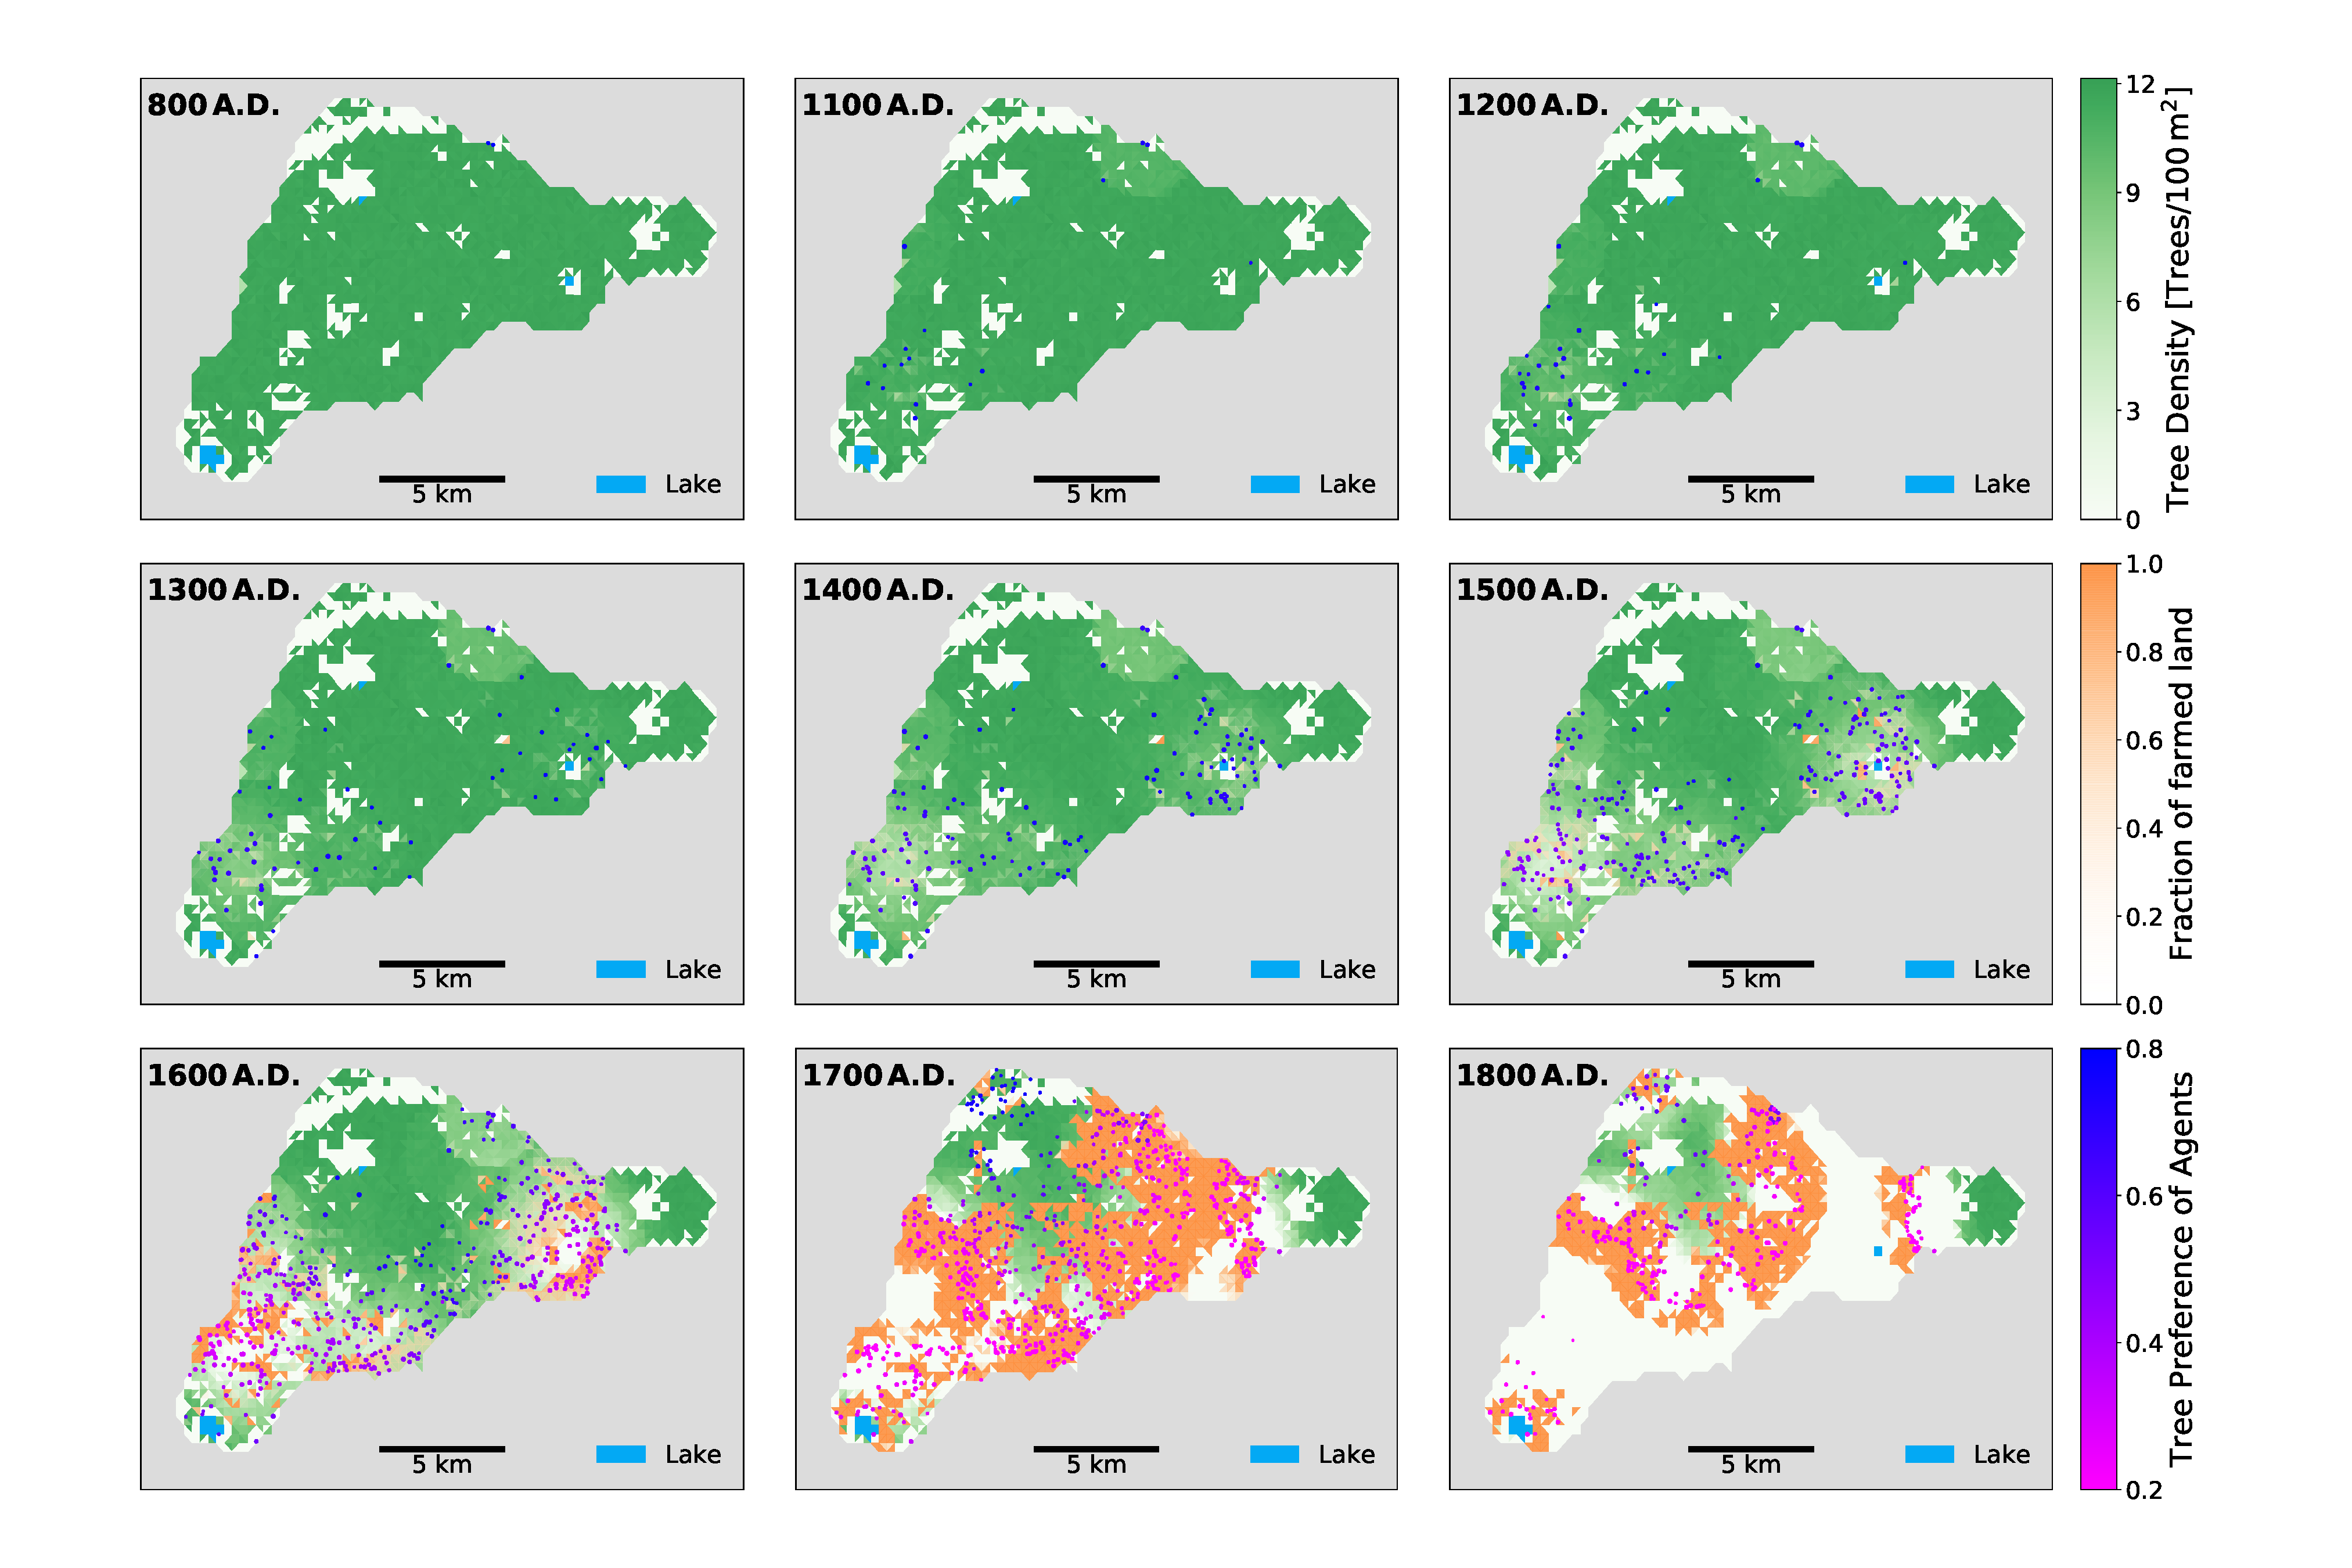
\includegraphics[width=\linewidth]{../../Thesis/images/Results/Standard/Rull2020_Comparison_seed3}}
	\end{minipage}
%\end{columns}
%\only<4>{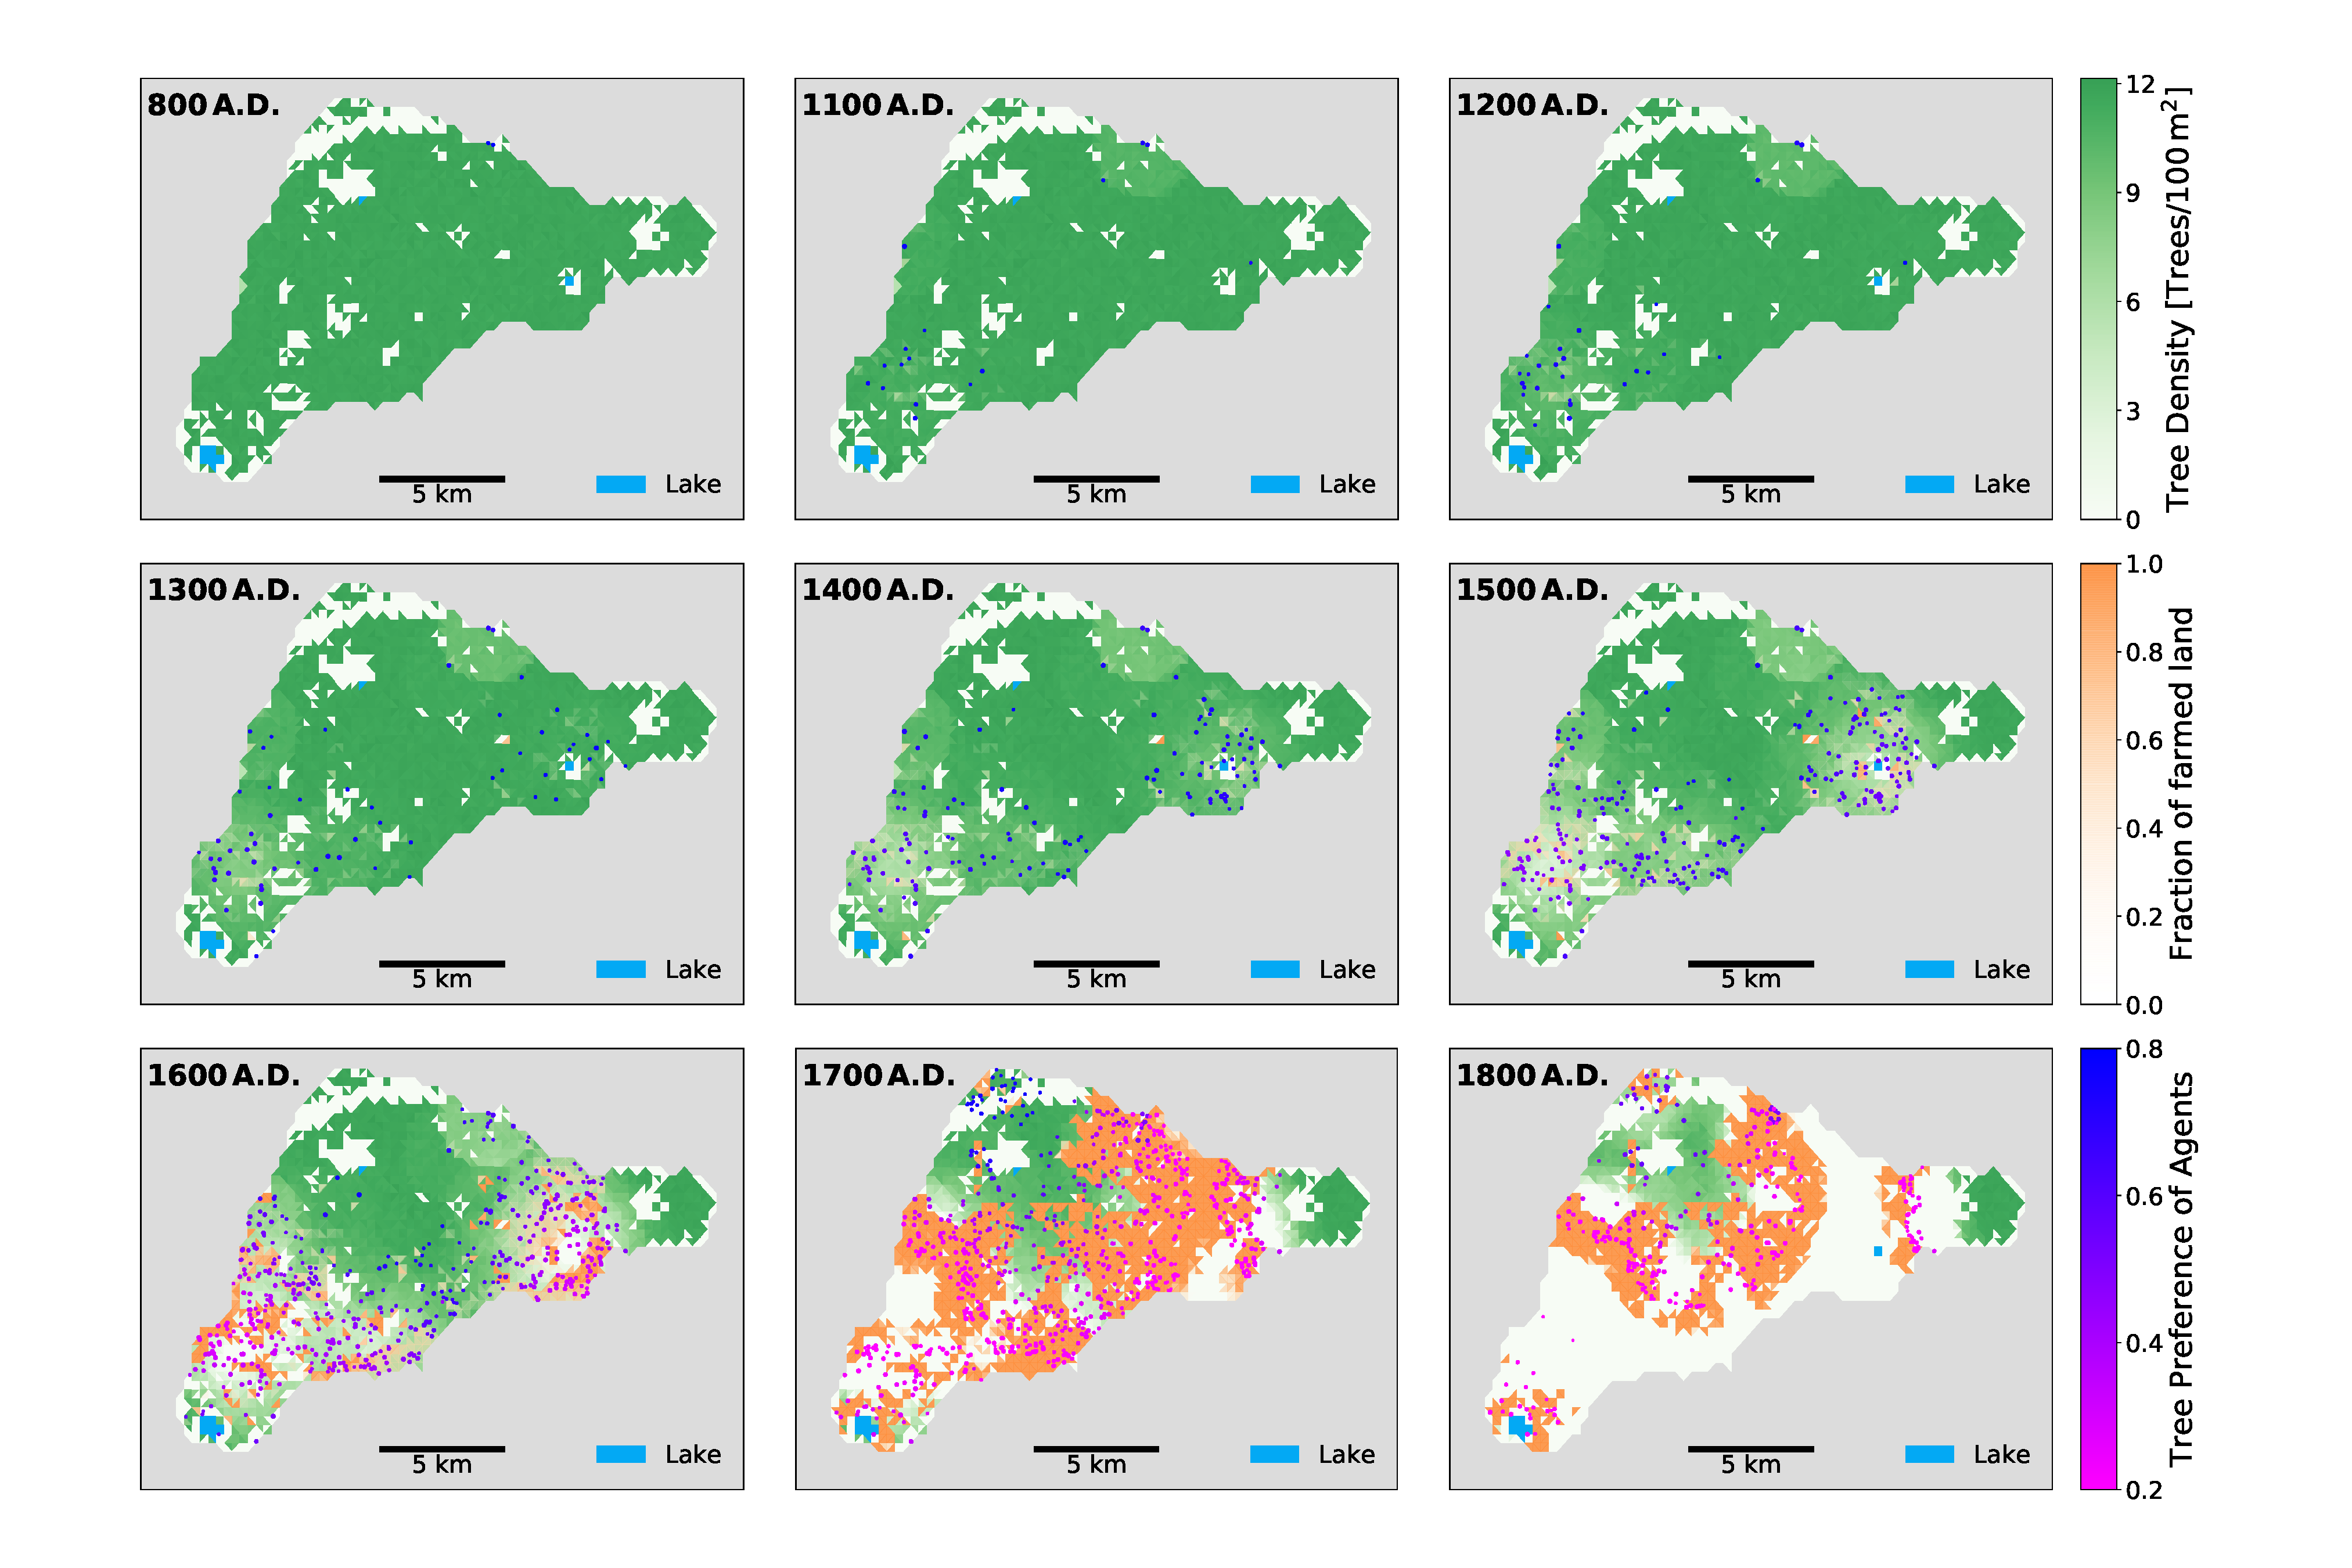
\includegraphics[width=0.87\linewidth]{../../Thesis/images/Results/Standard/Rull2020_Comparison_seed3}}

\end{frame}

%\begin{frame}{Result 1: Spatial Patterns and Comparison with Sediment Data}
%\centering
%\only<1>{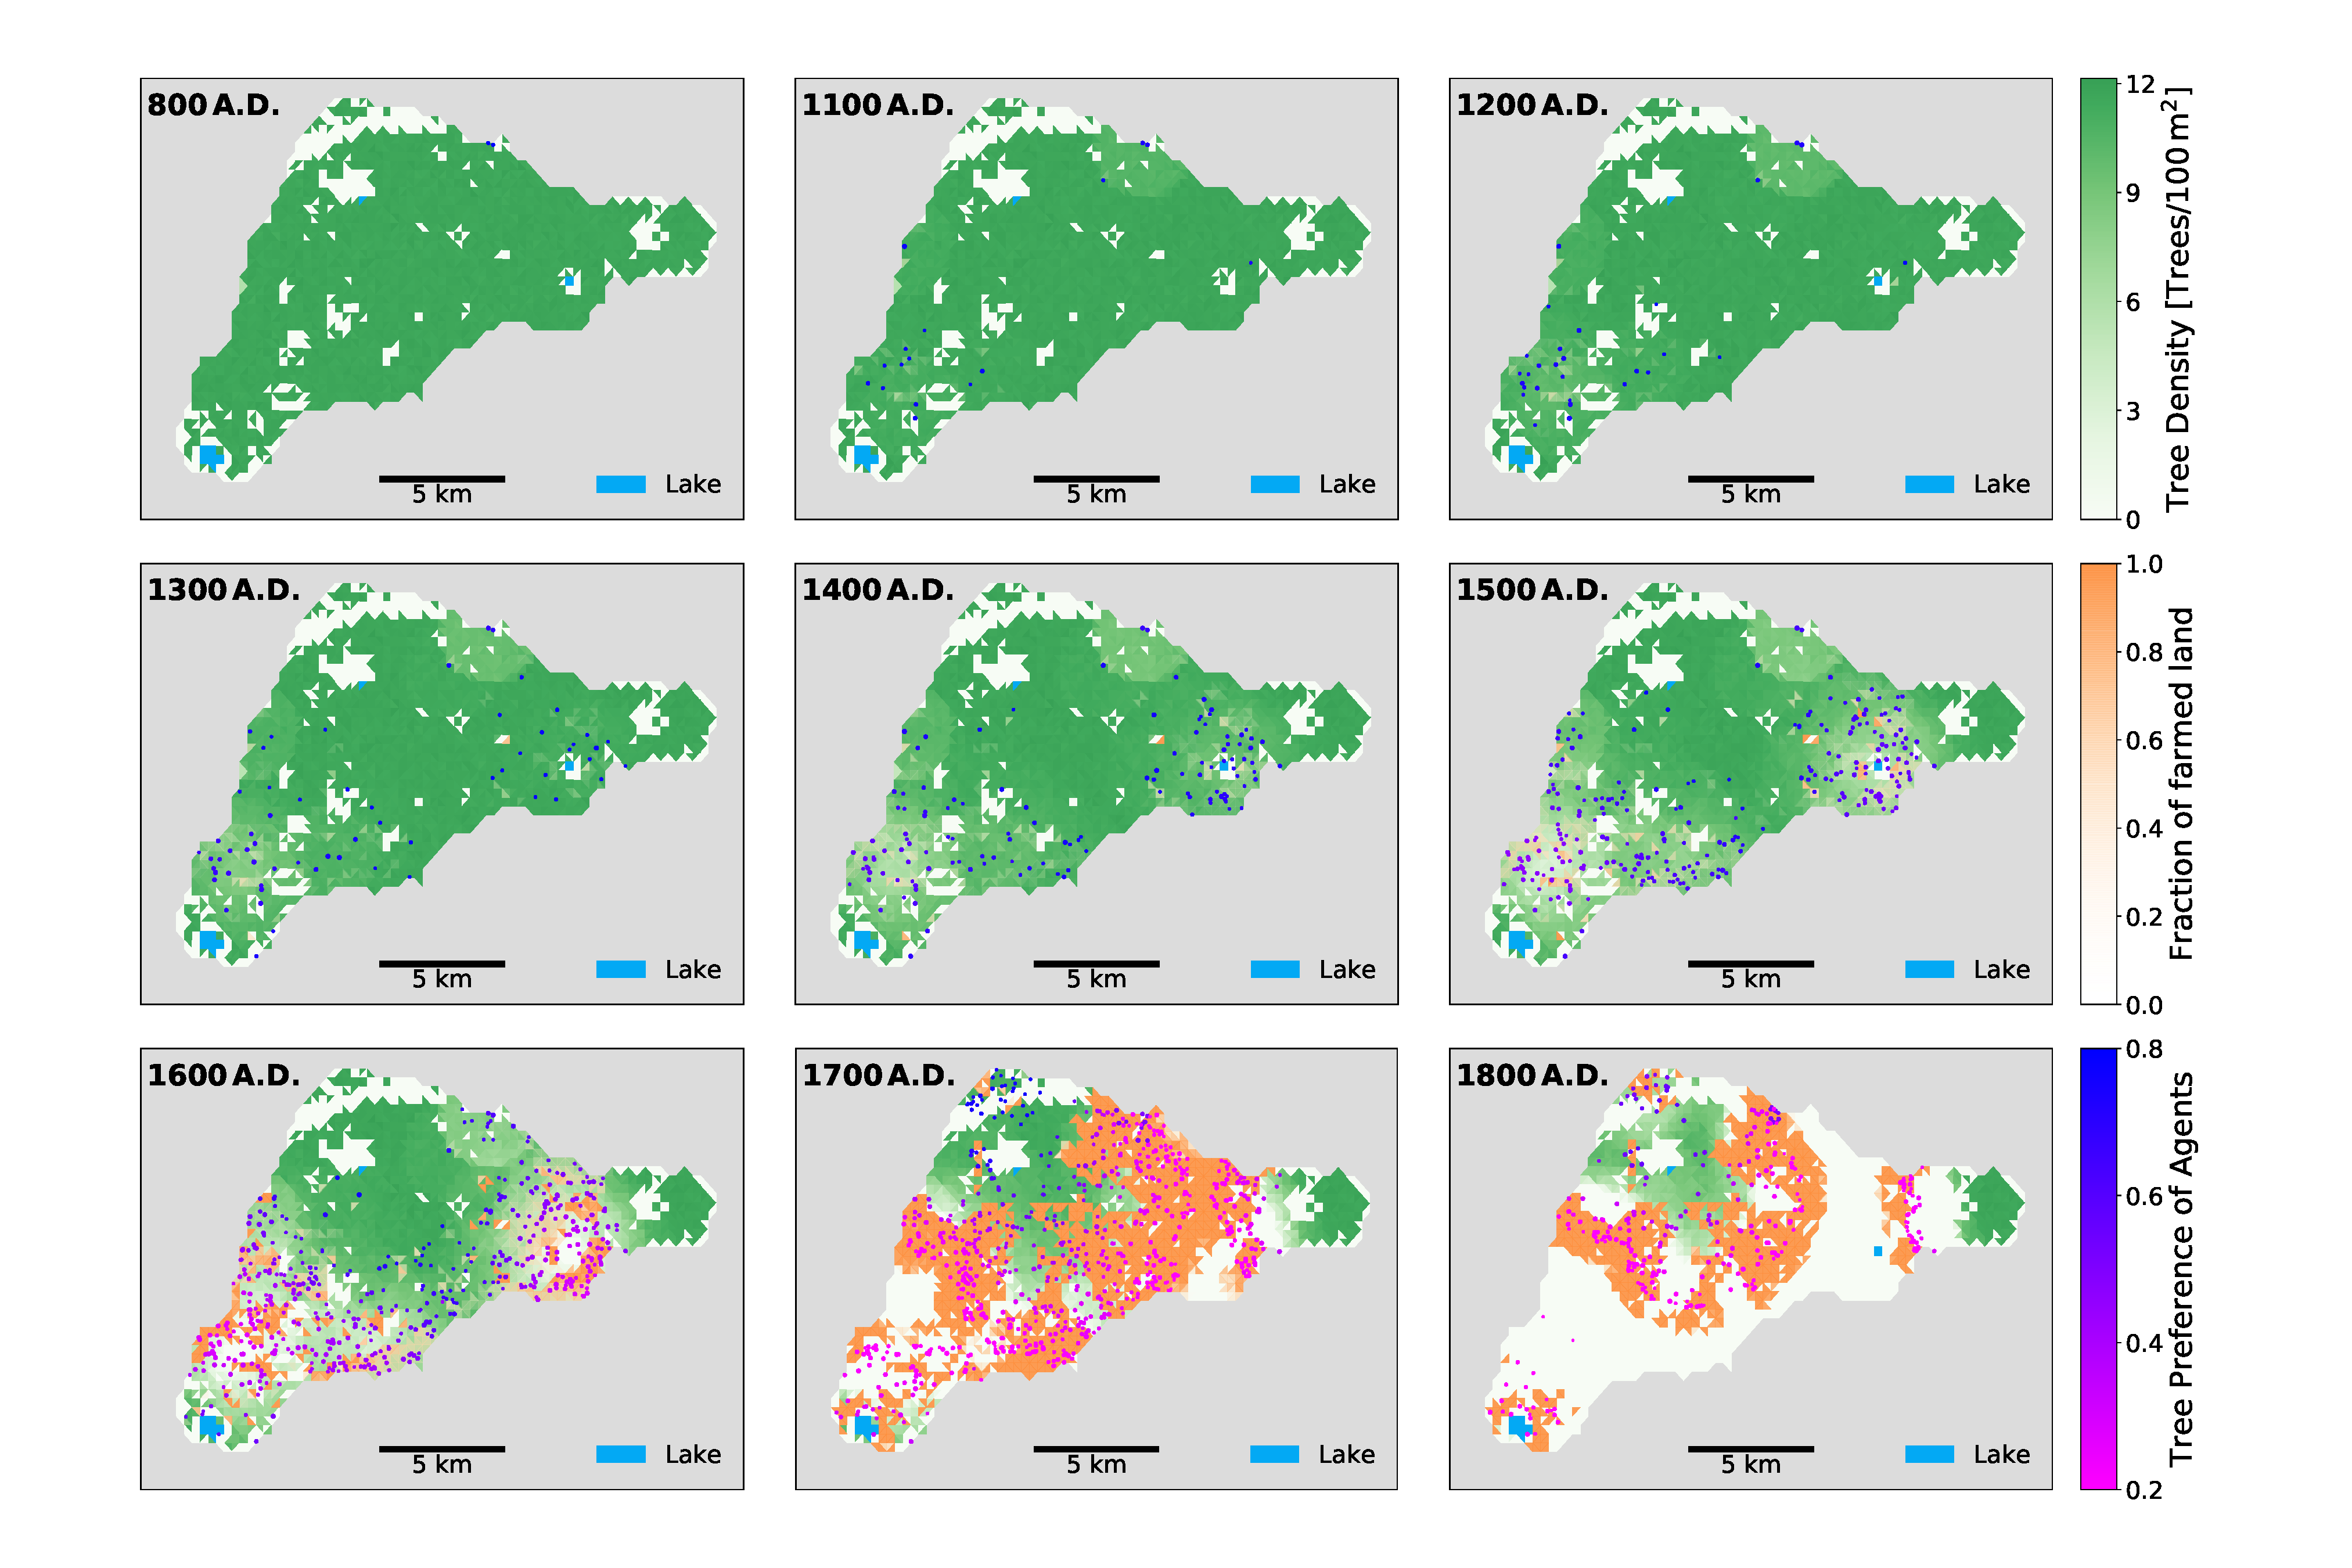
\includegraphics[width=0.8\linewidth]{../../Thesis/images/Results/Standard/Rull2020_Comparison_seed3}}
%\only<2>{
%\begin{figure}
%\begin{subfigure}{0.48\textwidth}
%	\centering	
%	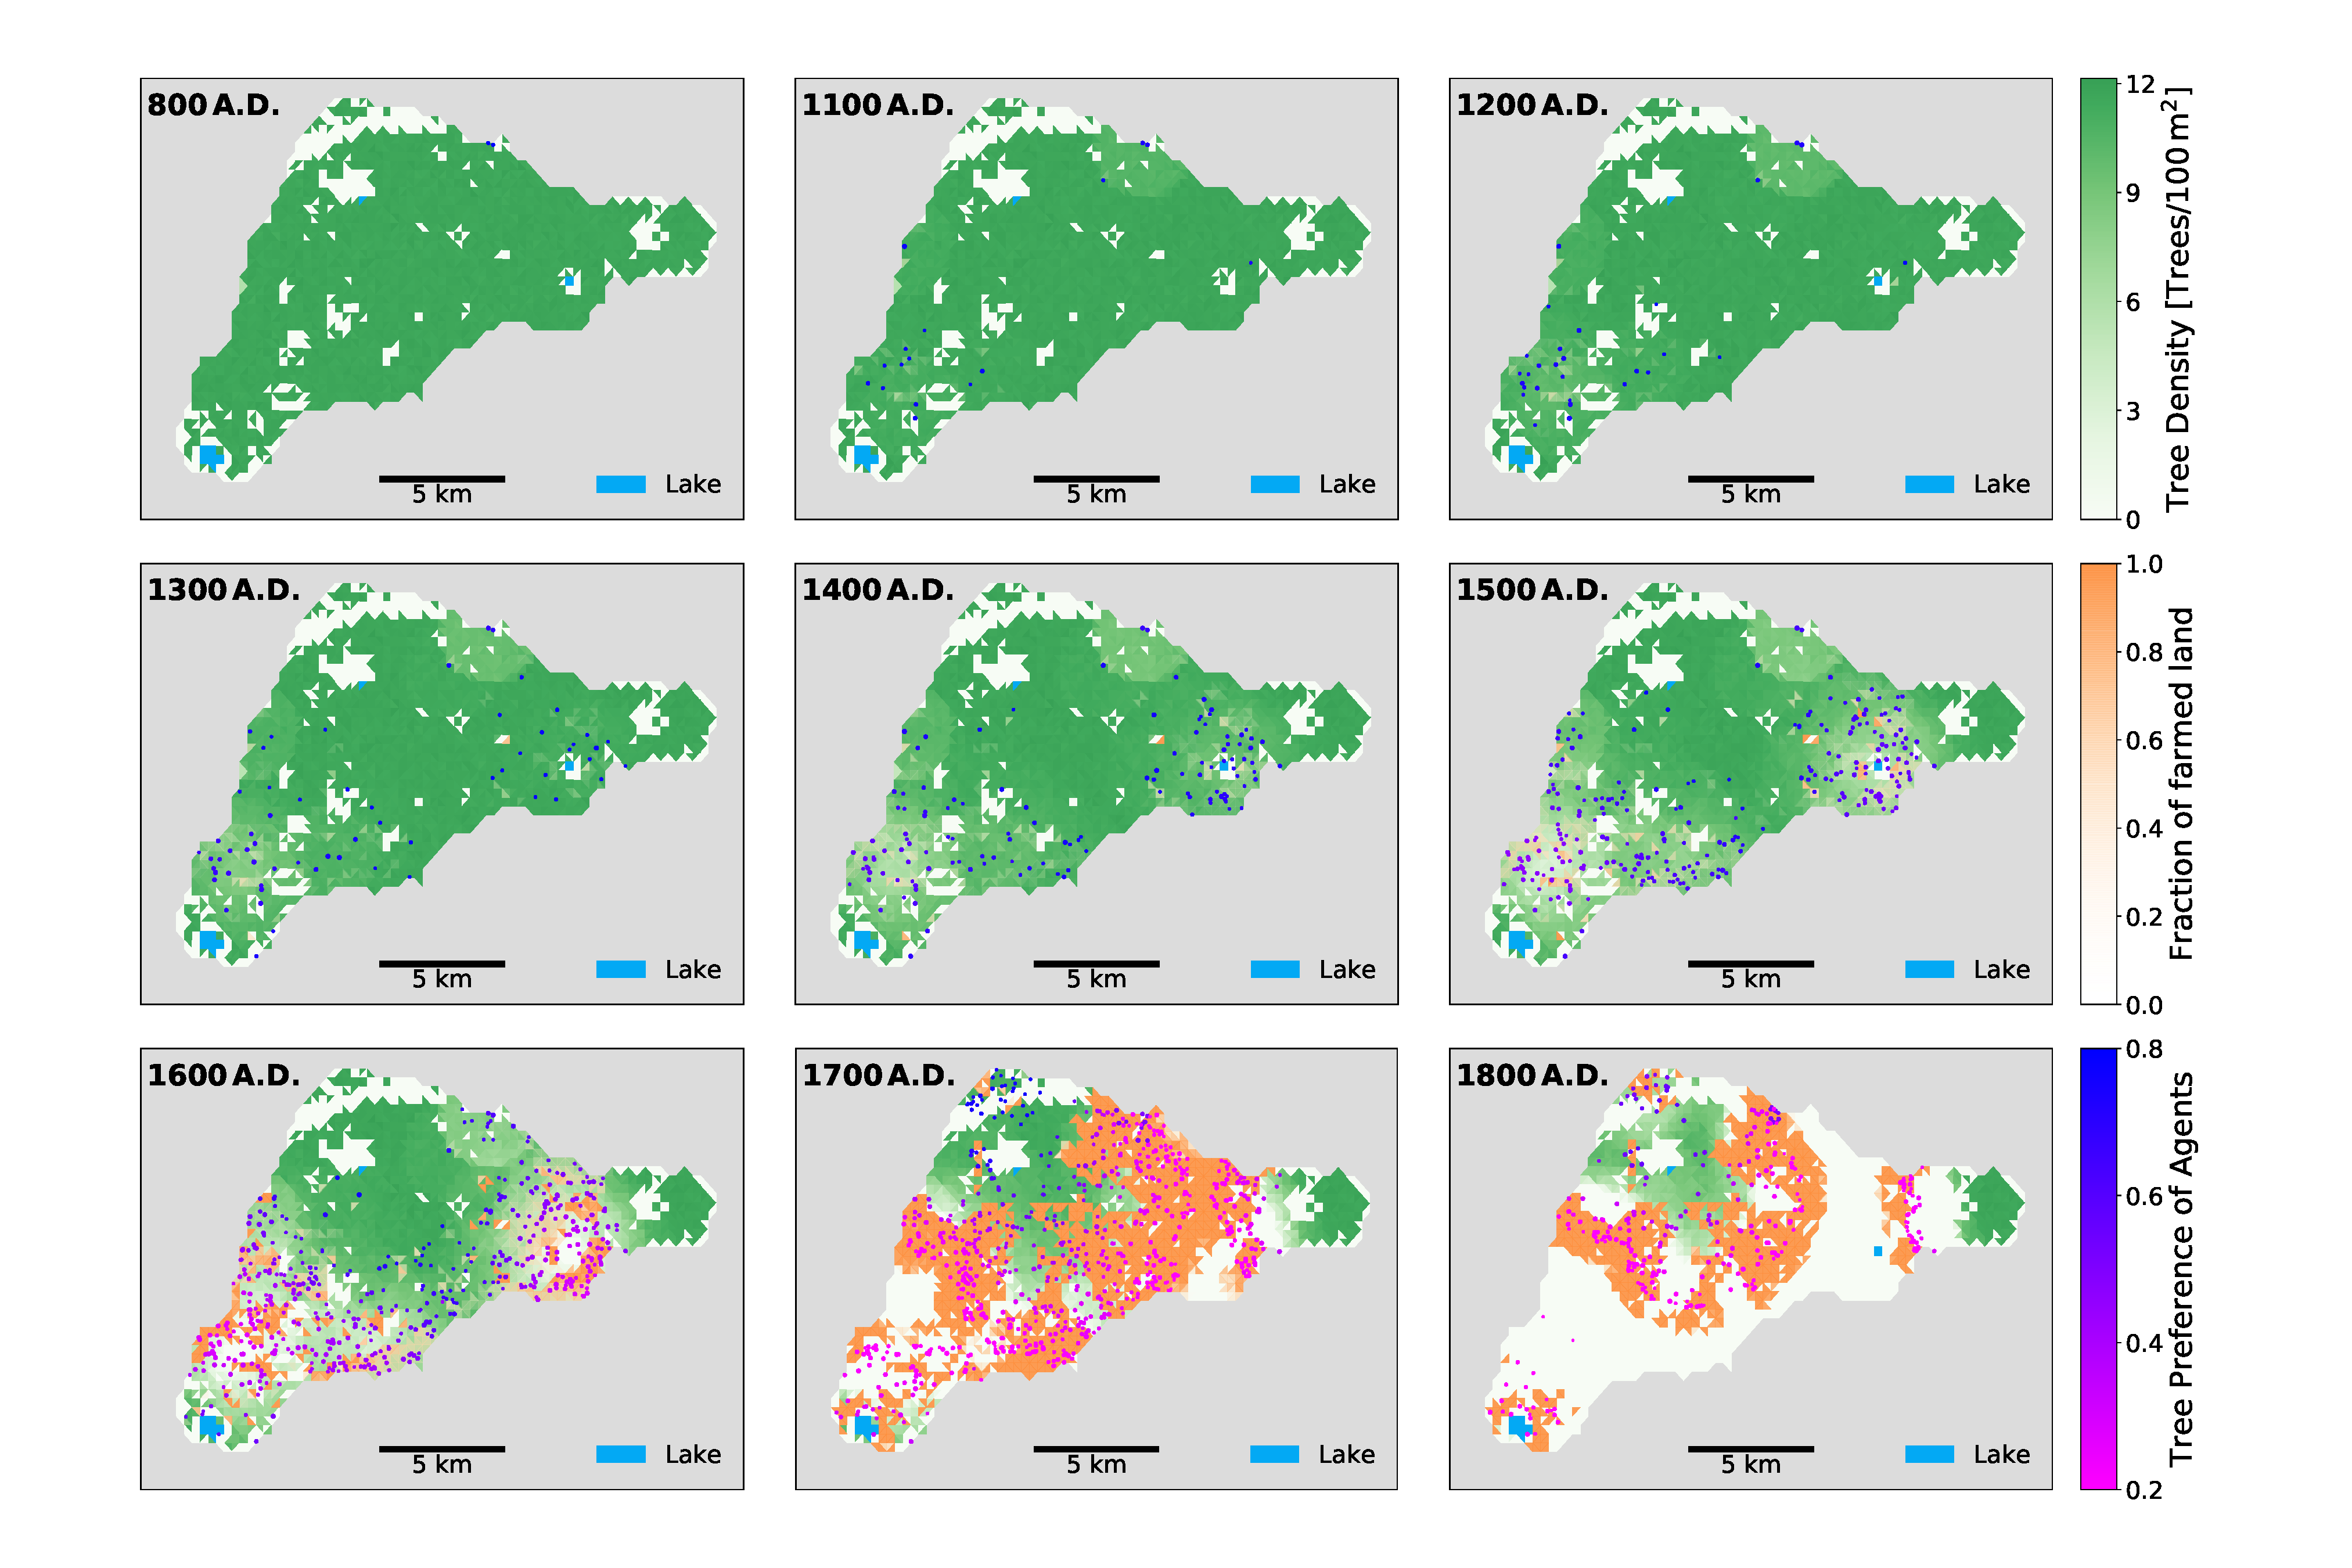
\includegraphics[width=\linewidth]{../../Thesis/images/Results/Standard/Rull2020_Comparison_seed3}
%\end{subfigure}
%\begin{subfigure}{0.48\textwidth}
%	\centering		
%	\includegraphics[width=\linewidth]{../../RullFigure/Rull2020Pattern_small}
%	\caption{\citet{Rull2020}}
%\end{subfigure}
%\end{figure}
%}
%\end{frame}


\begin{frame}{Different Environmental Conditions \& Myopic Agents}
\centering
\only<1>{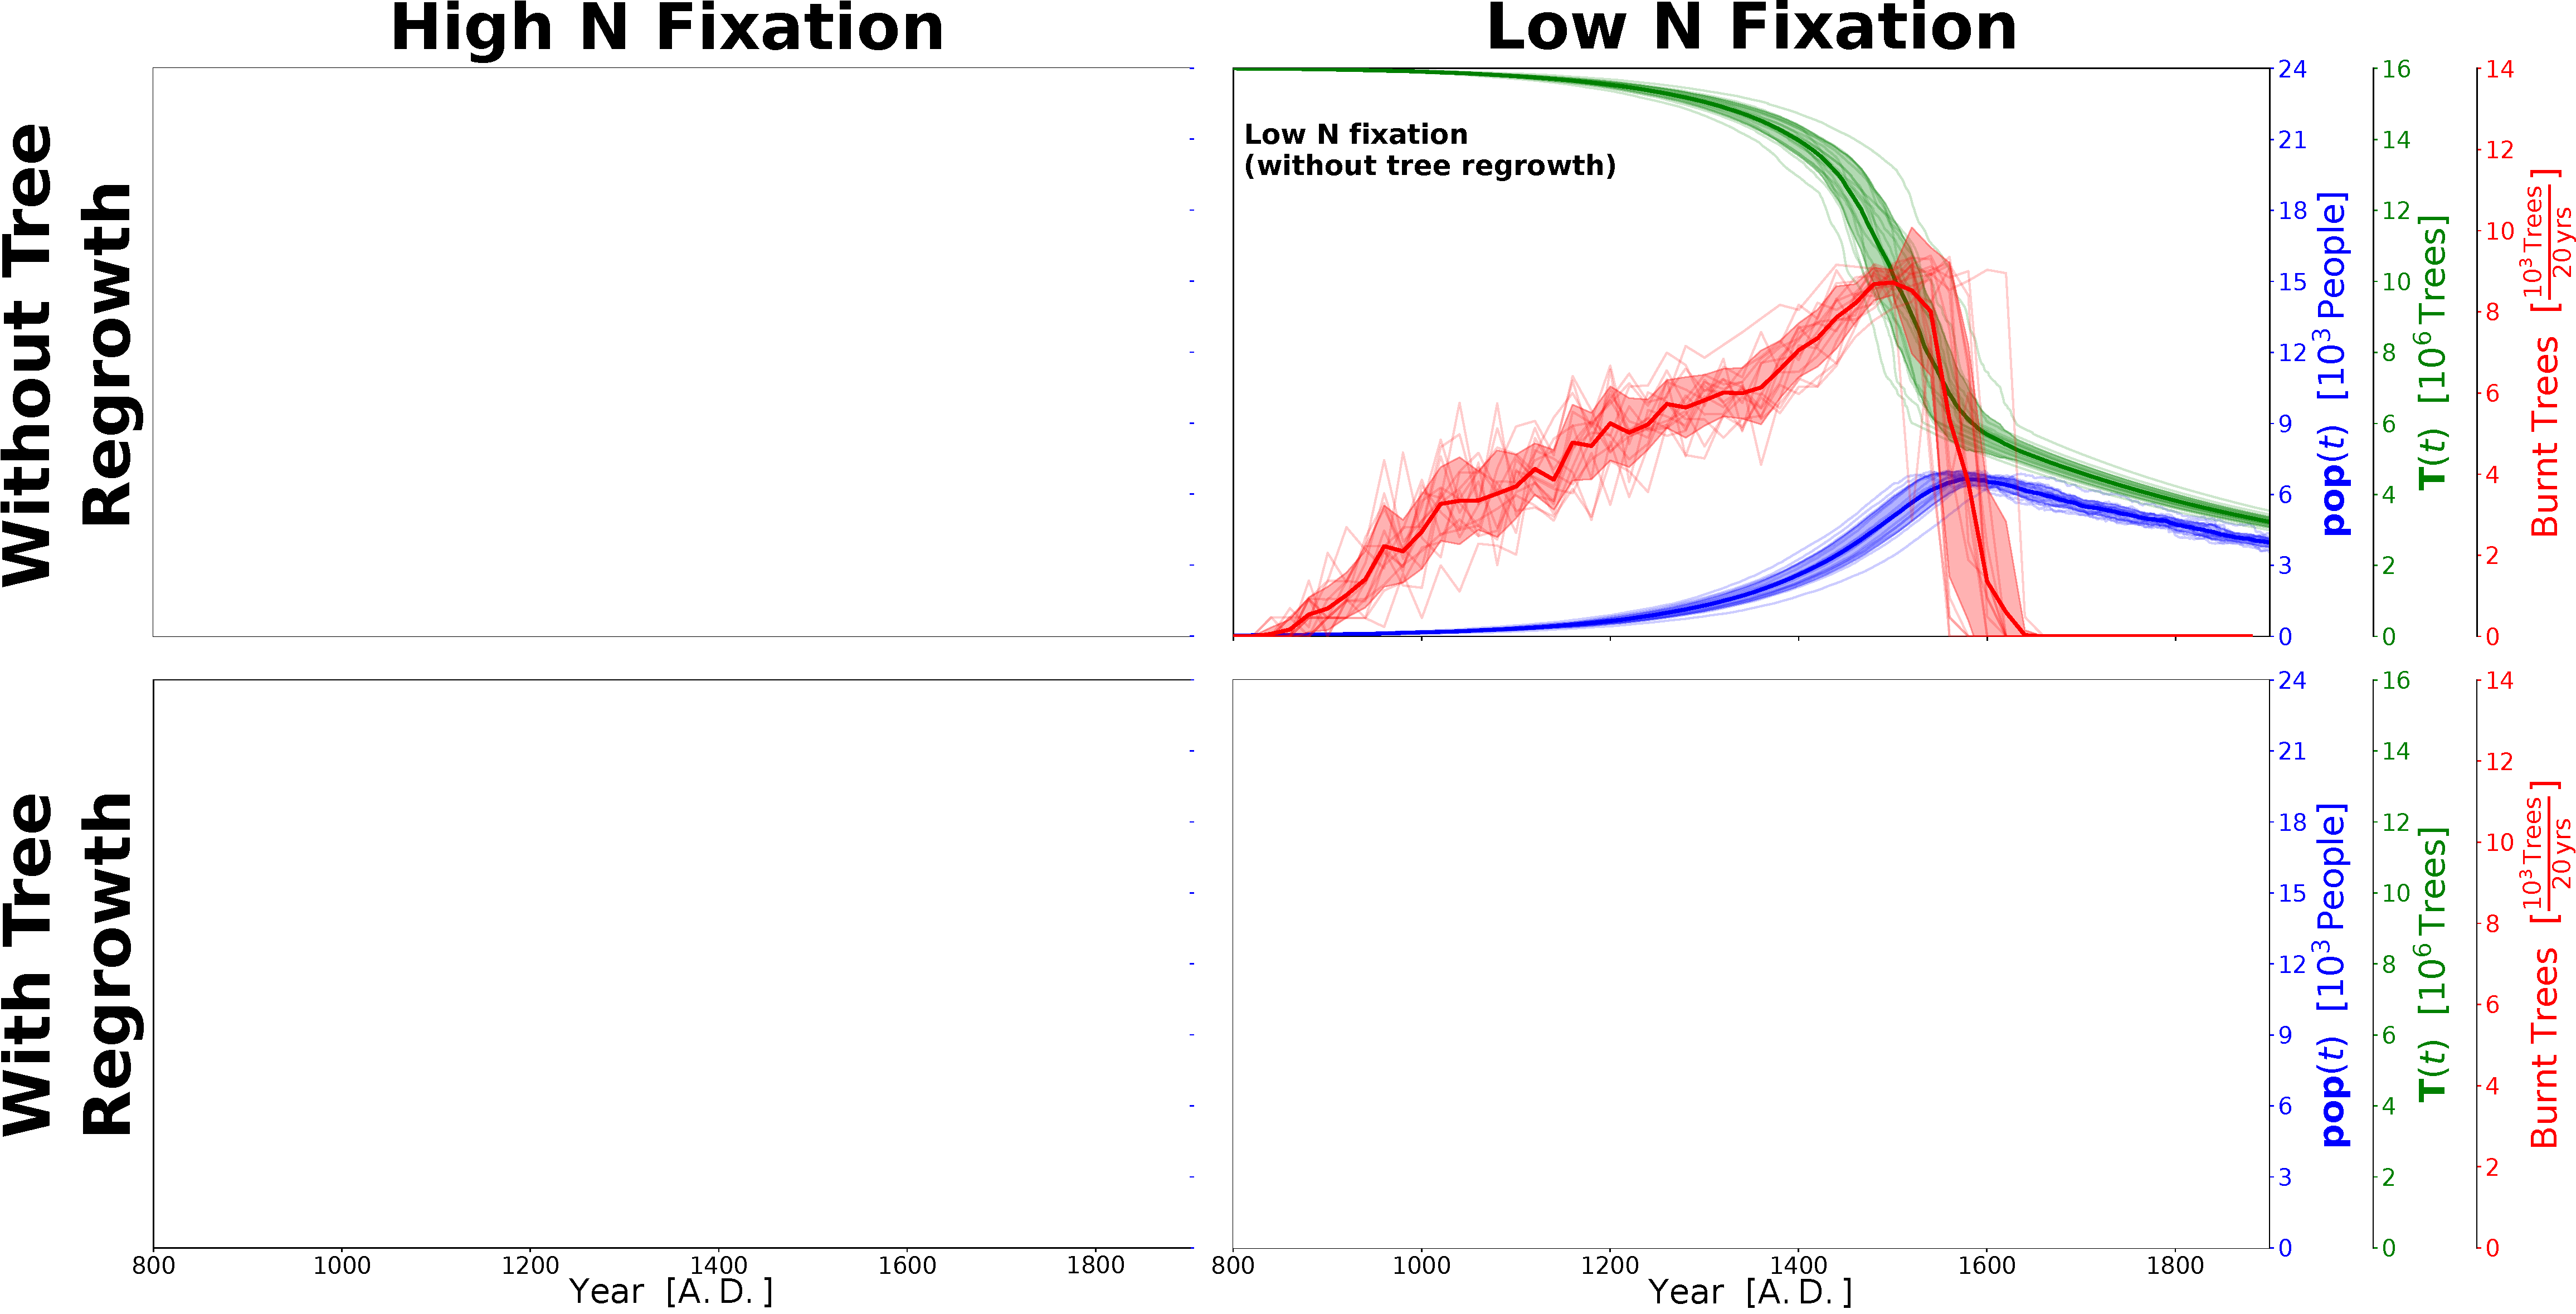
\includegraphics[width=1\linewidth]{../../Thesis/images/Results/Standard/EnsembleStatistics_allTheories_presentation1}}
\only<2>{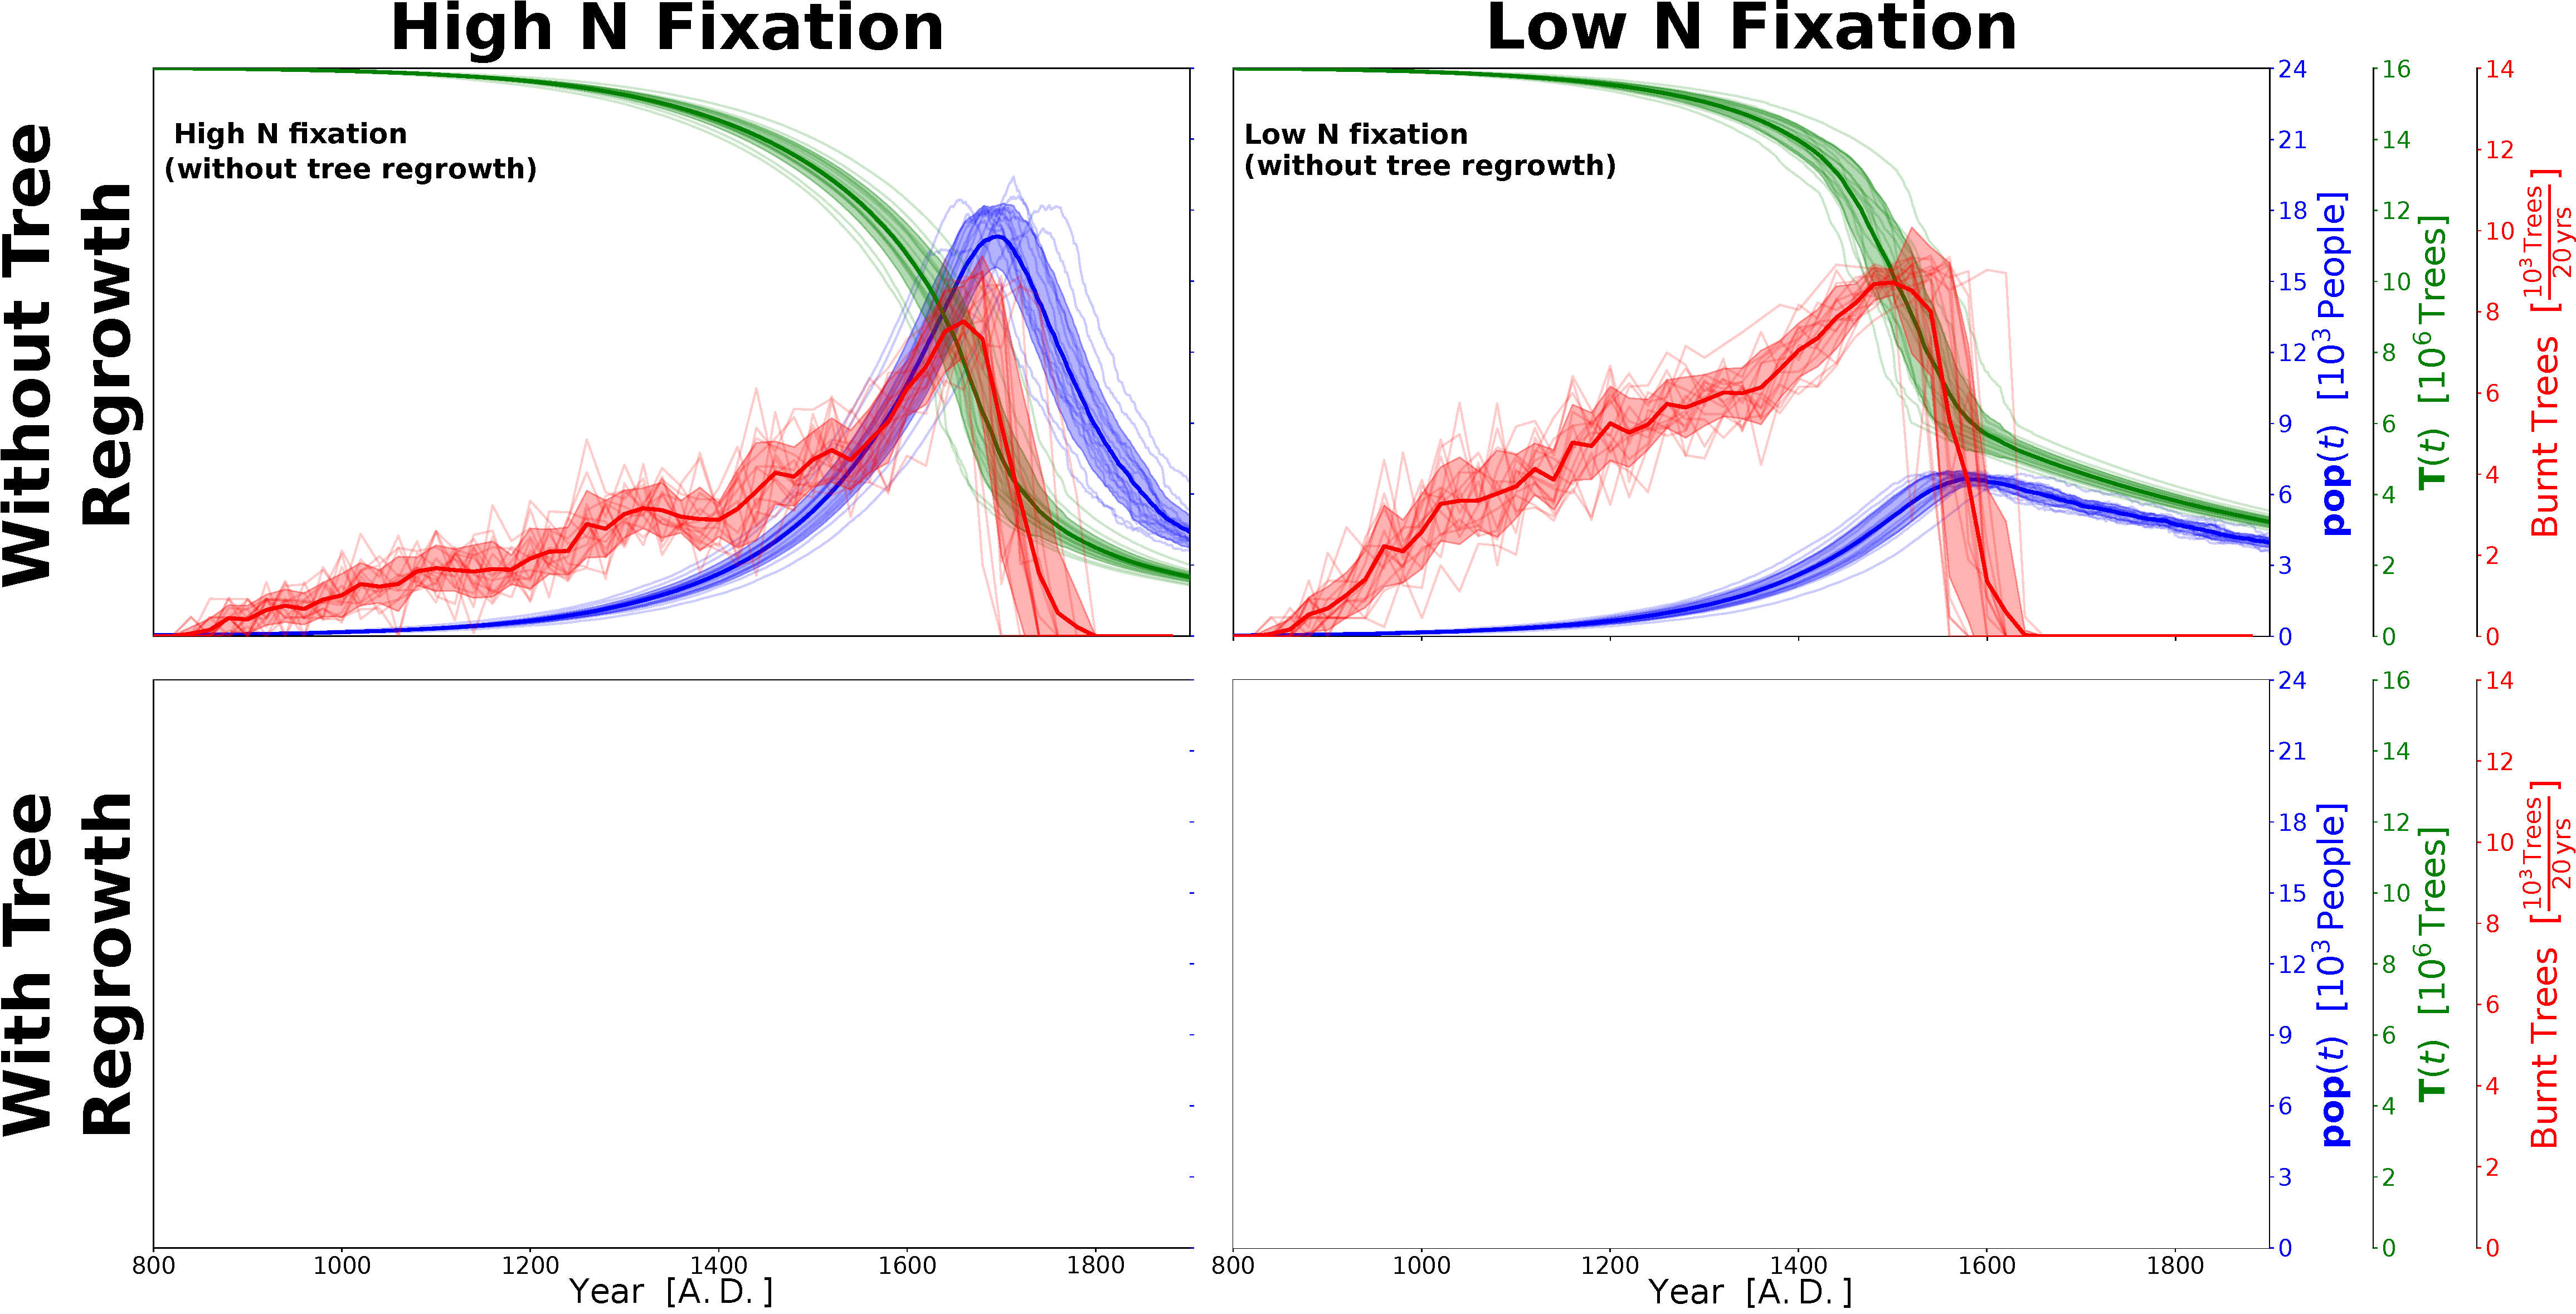
\includegraphics[width=1\linewidth]{../../Thesis/images/Results/Standard/EnsembleStatistics_allTheories_presentation2}}
\only<3>{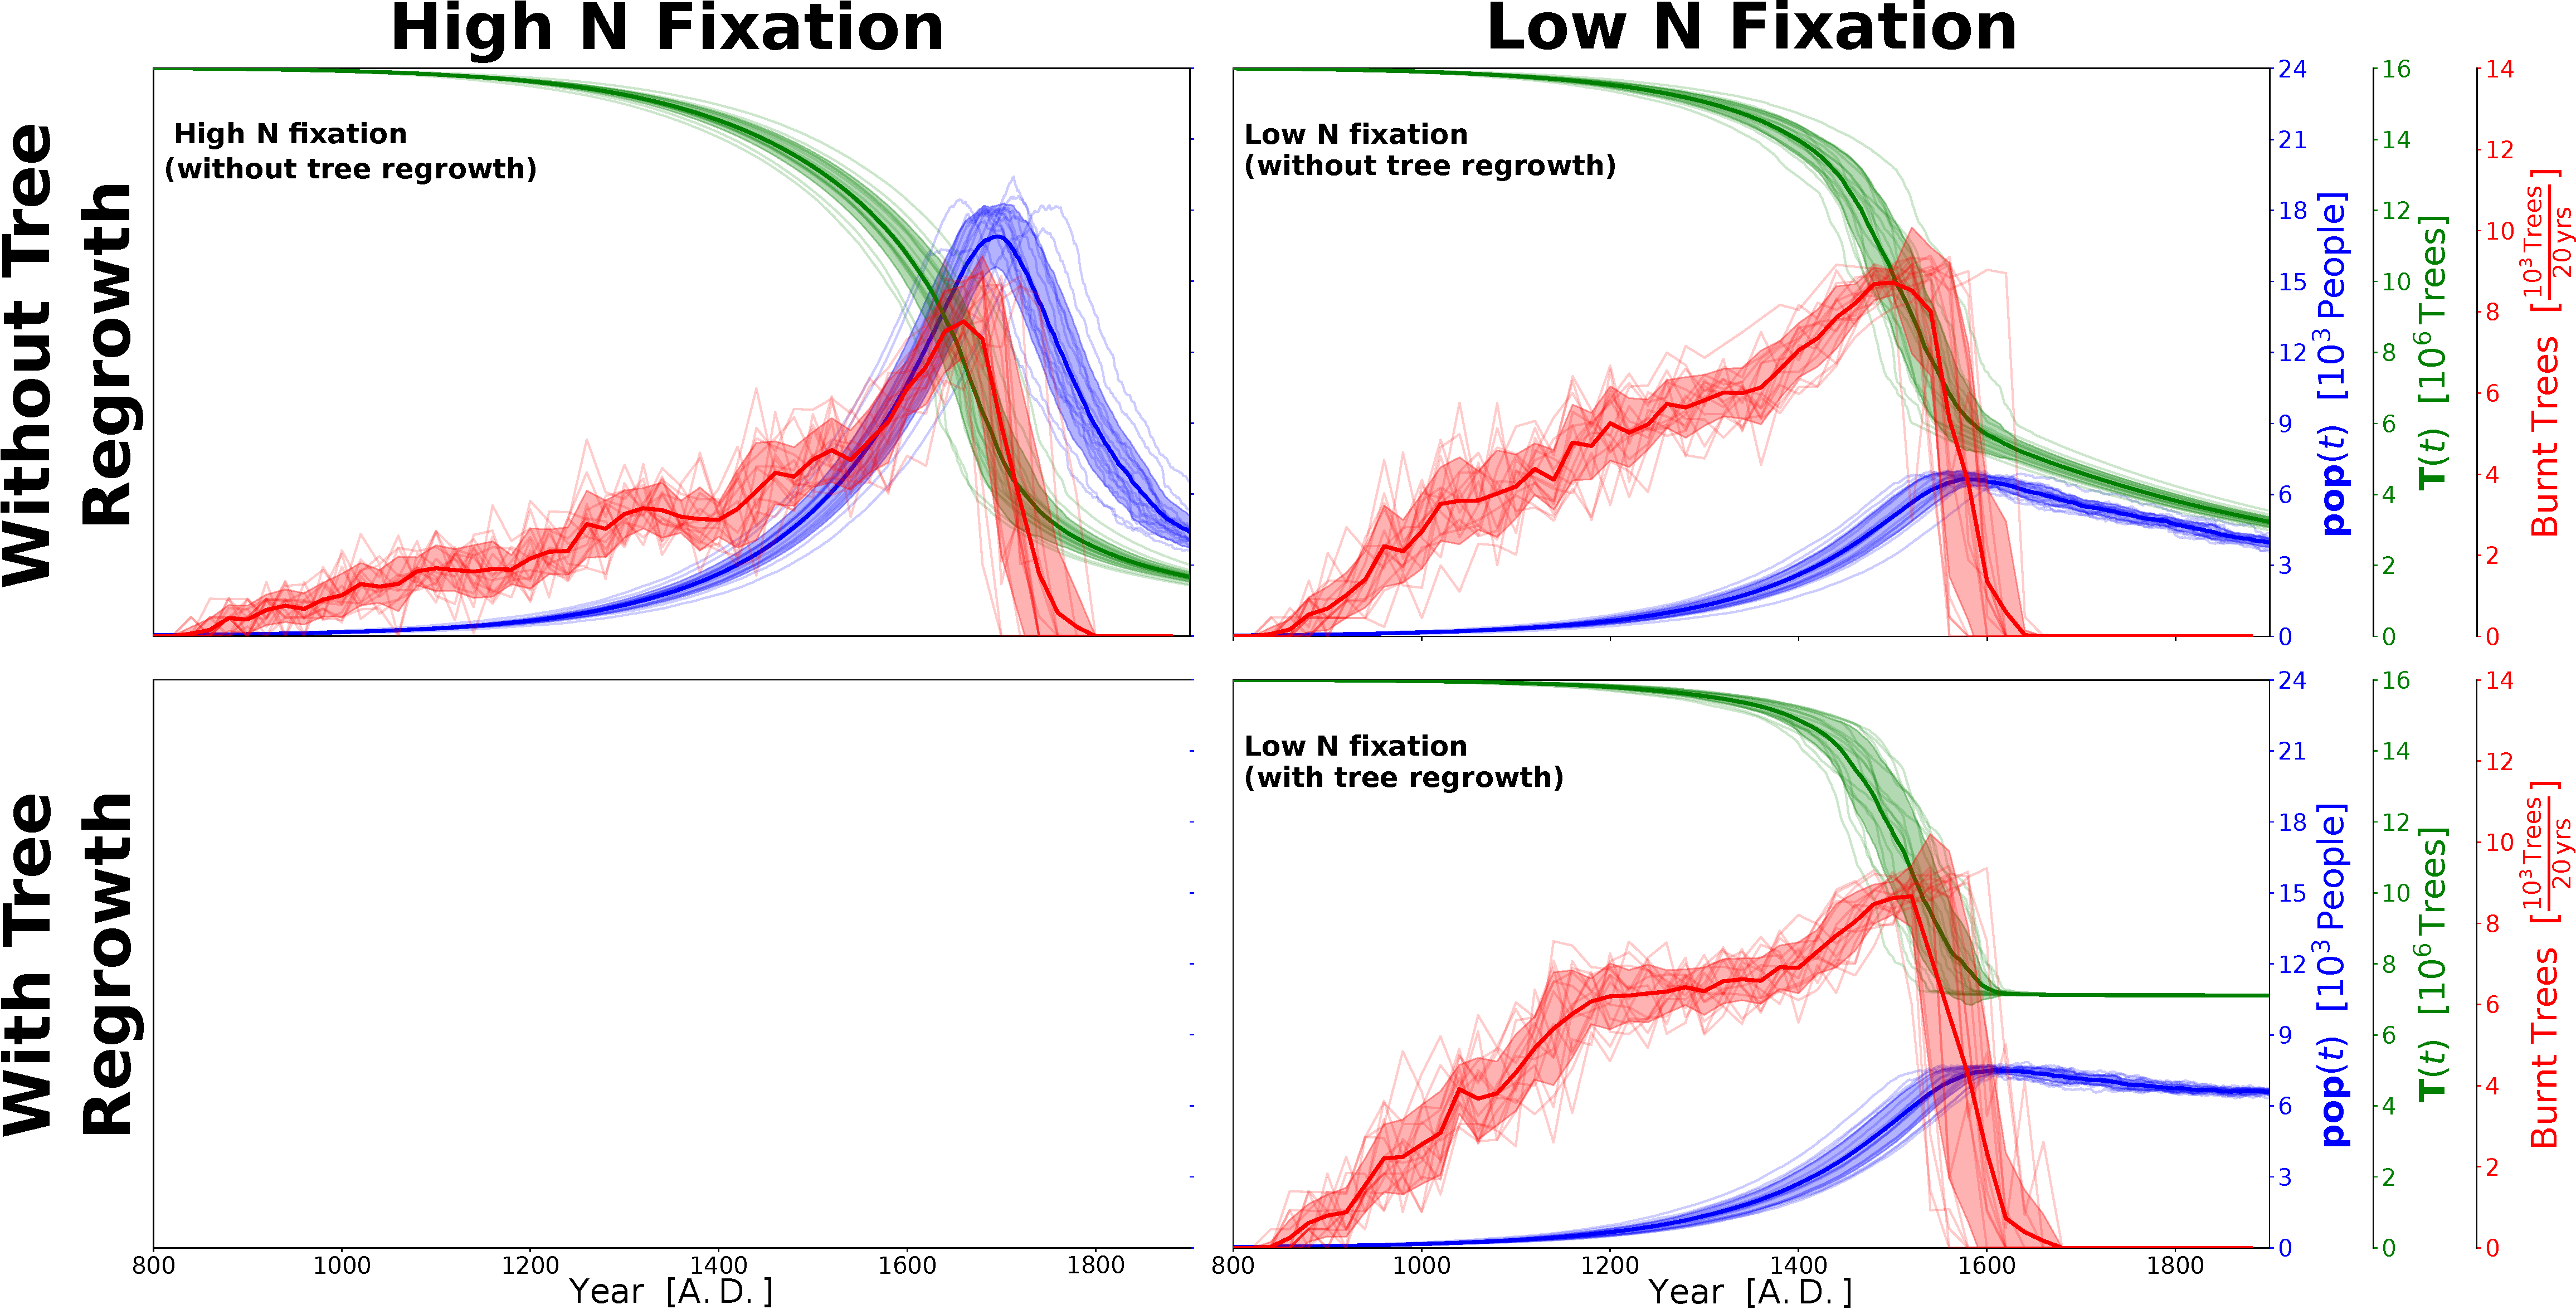
\includegraphics[width=1\linewidth]{../../Thesis/images/Results/Standard/EnsembleStatistics_allTheories_presentation3}}
\only<4>{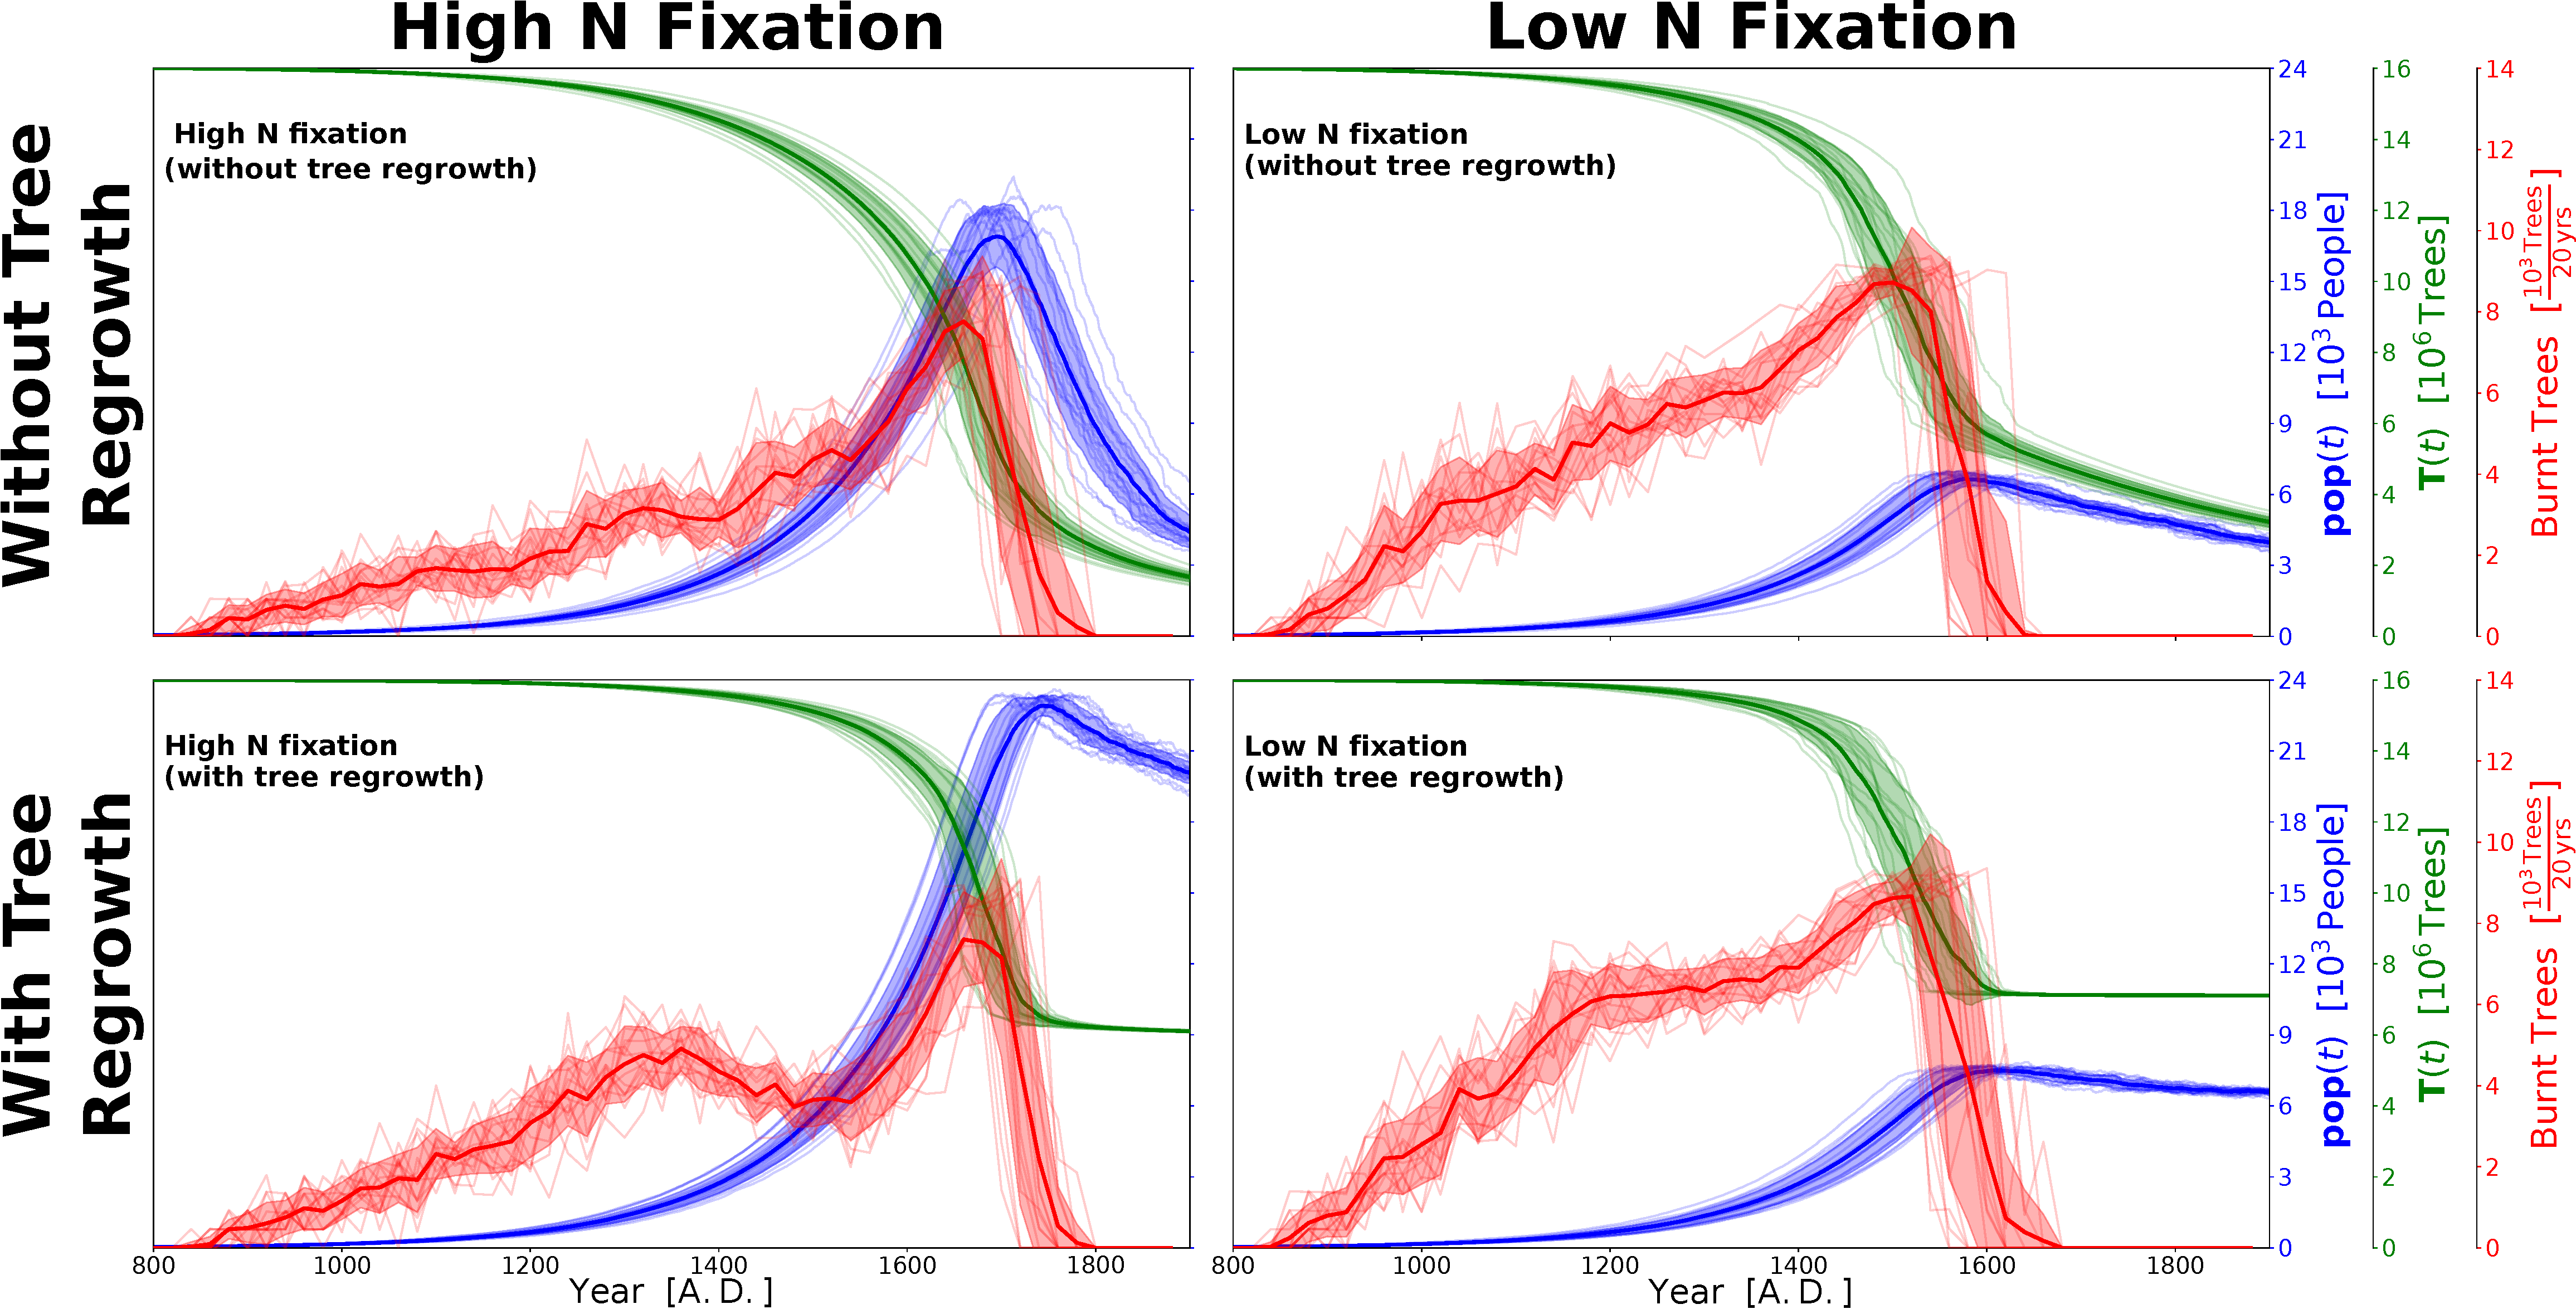
\includegraphics[width=1\linewidth]{../../Thesis/images/Results/Standard/EnsembleStatistics_allTheories_presentation}}
\end{frame}




\begin{frame}{Dynamics in Separate Regions}
\centering
\only<1>{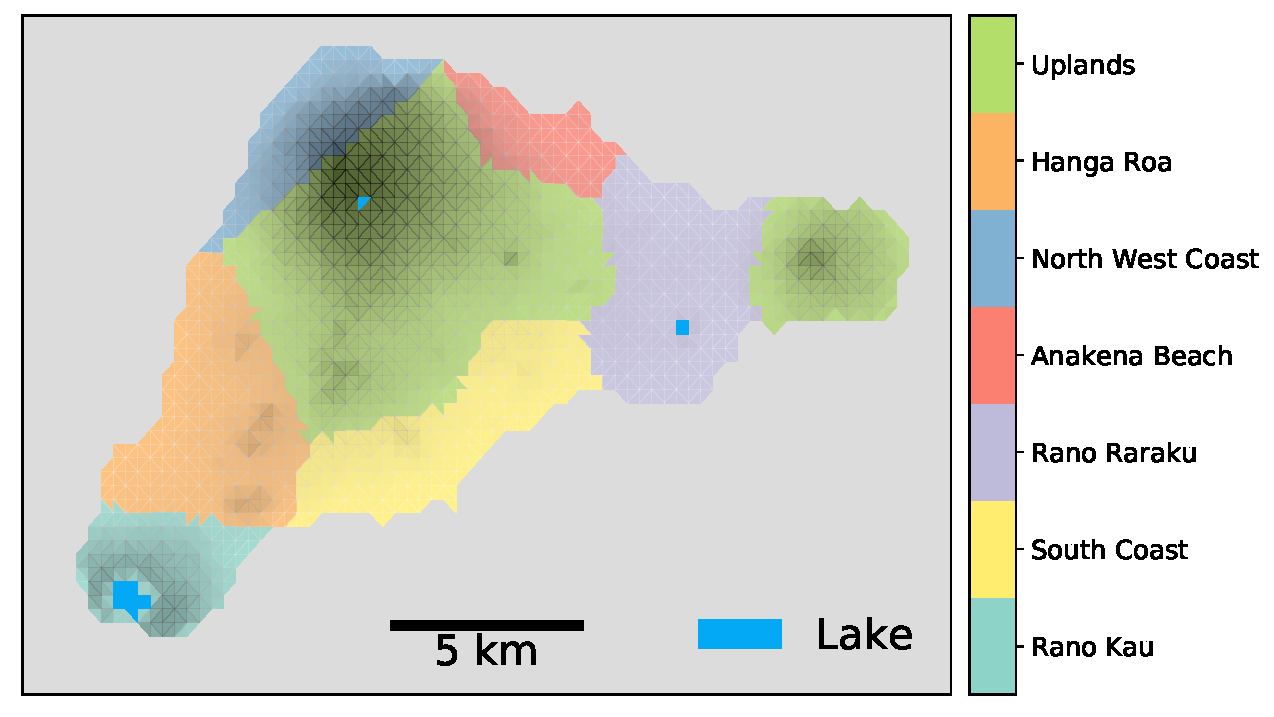
\includegraphics[width=0.8\linewidth]{../../Thesis/images/Results/Standard/MapRegionsCoarse}}

\only<2>{ {\scriptsize
	Environmental conditions: High N fixation and without tree regrowth}\\ 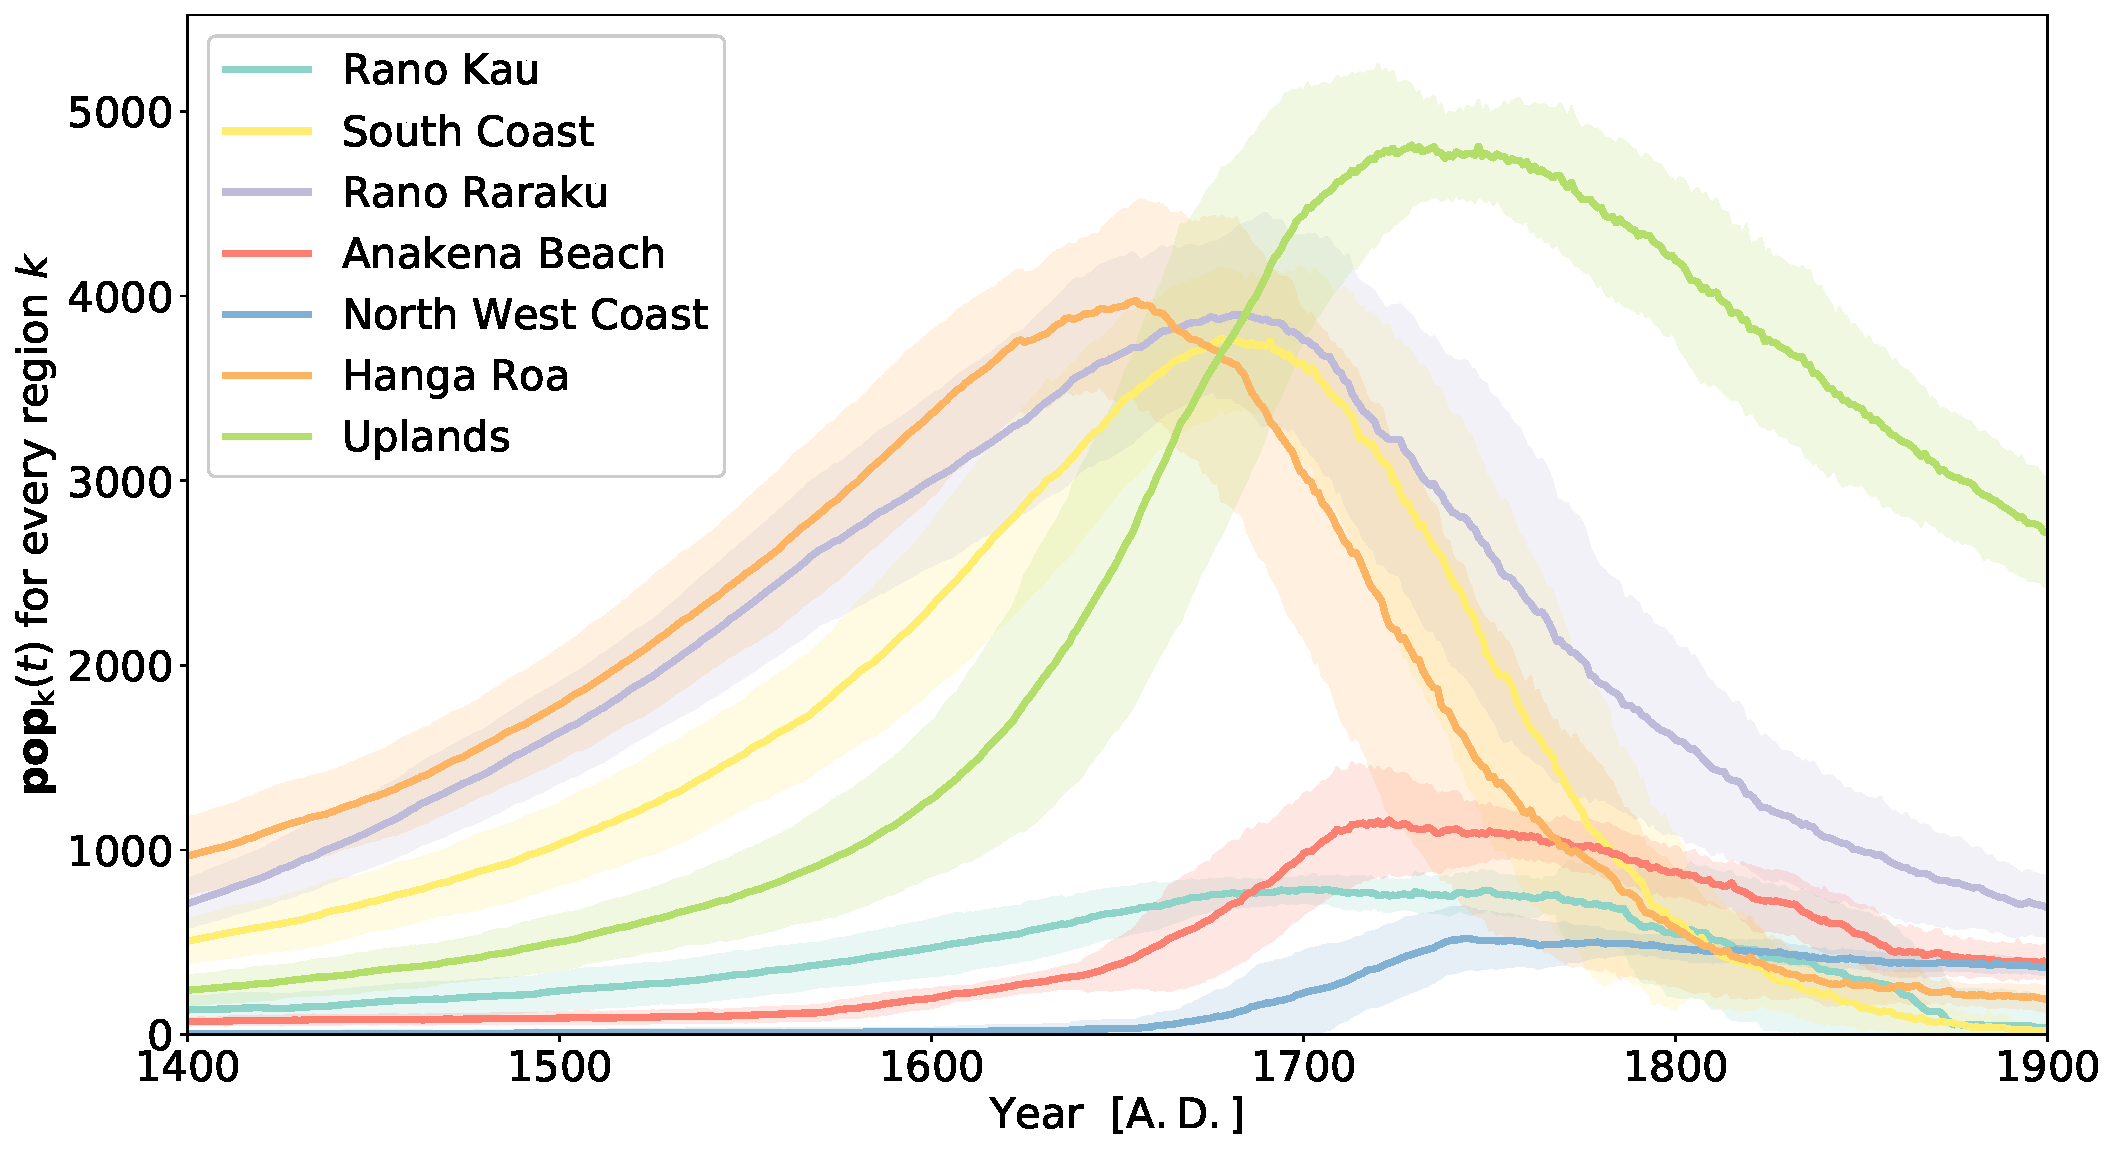
\includegraphics[width=0.8\linewidth]{../../Thesis/images/Results/Standard/RegionalStatsEnsembleOnly.pdf}
\\
\ra Heterogeneous regional dynamics!
}
\end{frame}

\begin{frame}{Further Results}
\centering
\begin{itemize}
%\pause\item Reason for Population decline is local variability 
\pause\item Microscopic spatial confinement is crucial for aggregate dynamics
\pause\item Strategy to adapt to environmental degradation: Early, slow adaptation better than late, fast adaptation! %The earlier, the `better'
\pause\item Moving strategy impacts both spatial AND aggregate temporal patterns
%\pause\item 
\end{itemize}
\end{frame}
